\chapter{On-Site Commissioning}
\label{chap:commissioning}
\chaptoc{}

% ########################################

\newpage
\section{Introduction}
\label{sec:commissioning_intro}
\begin{colsection}

In this chapter I describe \todo{TODO}.
%
\begin{itemize}
    \item In \todo{A SECTION} I describe \todo{SOMETHING}.
\end{itemize}
%
All work described in this chapter is my own, and has not been published anywhere else.

\end{colsection}

% ########################################

\newpage
\section{Deploying the hardware}
\label{sec:deployment}
\begin{colsection}

% ~~~~~~~~~~~~~~~~~~~~

\begin{colsection}

\todo{WIP}

\end{colsection}

% ~~~~~~~~~~~~~~~~~~~~

\subsection{Deployment timeline}
\label{sec:timeline}
\begin{colsection}


\begin{figure}[p]
    \begin{center}
        \begin{tabular}{cl|@{\tls}l} %chktex 44
            2015 & July      & Collaboration meeting in Warwick (29 Jul) \\
                 & September & Research collaboration agreement signed \\
                 &           & \textit{First observation of gravitational waves (GW 150914)} \\
            \midrule
            2016 & September & La Palma site construction begins \\
                 & November  & First dome assembled \\
                 &           & \textit{LIGO second observing run (O2) begins} \\
            \midrule
            2017 & March     & \textcolor{Blue}{Trip 1 (23--31 Mar) --- install dome systems} \\
                 & May       & Telescope hardware installed \\
                 & June      & \textbf{GOTO first light (19 Jun)} \\
                 &           & Collaboration meeting in Warwick (19--20 Jun) \\
                 &           & \textcolor{Blue}{Trip 2 (22 Jun--7 Jul) --- install control software} \\
                 & July      & Inauguration ceremony (3 July) \\
                 &           & \textcolor{Blue}{Trip 3 (20--28 Jul) --- pilot commissioning} \\
                 &           & Robotic operations begin \\
                 &           & Dec motor drive fails \\
                 & August    & UT3 mirrors sent back to factory \\
                 &           & \textit{First gravitational wave counterpart detected (GW 170817)} \\
                 &           & \textit{O2 ends} \\
                 & November  & Drive motors upgraded \\
                 &           & Arm extensions installed \\
                 &           & \textcolor{Blue}{Trip 4 (9--16 Nov) --- on-site monitoring} \\
                 & December  & Second dome assembled \\
            \midrule
            2018 & January   & \textcolor{Blue}{Trip 5 (14 Jan--5 Feb) --- on-site monitoring} \\
                 & April     & Collaboration meeting in Warwick (11--13 Apr)\\
                 & May       & On-site monitoring program ends \\
                 & June      & Refurbished mirrors reinstalled, UT4 mirrors sent back \\
                 & July      & \textcolor{Blue}{Trip 6 (5--13 Jul) --- software development} \\
                 & December  & \textit{LIGO-Virgo Engineering Run 13 (14--18 Dec)} \\
            \midrule
            2019 & February  & Refurbished mirrors reinstalled into UT3 \\
                 &           & Current 4-UT all-sky survey begins \\
                 & April     & \textit{LIGO-Virgo third observing run (O3) begins} \\
        \end{tabular}
    \end{center}
    \caption[Timeline of the GOTO project]{
        A timeline of the GOTO project from when I joined up until the time of writing, including the six trips I made to La Palma during commissioning (in \textcolorbf{Blue}{blue}) and concurrent developments in the field of gravitational waves (in \textit{italics}).
    }\label{tab:timeline}
\end{figure}

\clearpage

\end{colsection}

% ~~~~~~~~~~~~~~~~~~~~

\newpage
\subsection{Additional dome systems}
\label{sec:arduino}
\begin{colsection}

GOTO uses a dome manufactured by Astrohaven, the same company that made the pt5m dome \citep{pt5m}. Based on experience at Sheffield with p5tm, it was decided that some extra hardware was needed to be added to the dome in addition to the in-built system. For p5tm the entire dome control unit was replaced by a custom one designed and manufactured in Durham, however if possible we wanted to avoid such a drastic step. There were several limitations of the stock dome, which are outlined below.
%
\begin{itemize}
    \item First, there was no easily-accessible emergency stop button to cut power to the dome in an emergency (e.g.\ something gets caught in the motors). This is a serious concern for pt5m as when open the shutters completely cover the access hatch, making it dangerous for anyone to be passing through the hatch when the dome is moving. Therefore one of the additions to pt5m was an emergency stop button within arms reach of the hatch entrance. As the GOTO dome is taller the hatch is still mostly uncovered when the dome is open, however installing an emergency stop button was still a priority.
    \item In a similar health and safety concern, by default the dome does not come with a siren to sound when it opens or closes. This is an important safety feature when operating a robotic observatory, as the dome will be operated entirely through software and it is important to warn anyone on site several seconds before it is about to move. When members of the GOTO team are on-site the robotic systems can be disabled entirely by going into engineering mode (see \aref{sec:mode}), however it is still important to make sure there is no chance of the dome moving without prior warning. In addition, the GOTO site on La Palma is completely publicly accessible, and it is not unknown for tourists or hikers, or other astronomers, to be around the dome when it is unsupervised.
    \item By default the dome \glsfirst{plc} only provides limited information about the status of the dome shutters. As described in \aref{sec:dome}, the \gls{plc} only returns a single status byte in response to a query. This is not enough to distinguish whether the dome is fully or only partially open, and if one side is moving the status of the other side is unknown. It is possible to determine the current status by saving the previous status within the dome daemon, but having constant on/off switches would be more reliable.
    \item The dome comes with two in-built magnetic sensors on each side, which should detect when the shutters are either fully closed or fully open. However these have been know to be unreliable and tricky to align. In some cases the switches failed to trigger when the shutter reached its open limit, leading to the dome continuing to drive the belts and the shutter embedding itself into the ground. Therefore having secondary, independent sensors was a priority to ensure this did not happen.
    \item One final proposed addition was a quick-close button, which acts as a simple and direct way to communicate with the dome daemon. The motivation is a practical one: in the case that the weather turns bad and the telescope is exposed, assuming the automatic monitoring systems fail and we can't connect to close it remotely, it is a lot easier to direct someone on site to access the dome and press the prominent ``close'' button than direct them to log on to the in-dome computer, open a terminal and type \code{dome close}. In turn during the commissioning phase, when the software was still being tested and someone has to be on duty on-site all night, it is easiest if they have a single, simple button for them to press if they feel any rain. One requirement was that this button could not be easily confused with the emergency stop button (i.e.\ it should not be coloured red), as instead of stopping the dome this button will prompt it to move.
\end{itemize}
%
Adding an emergency stop button to the dome was fairly simple. As shown in \aref{fig:estop_plc} there was enough slack on the power cable for the PLC to install a prominent red button on the wall of the dome. When the button is pressed the power to the PLC is cut, which will prevent commands being sent to the dome motors and therefore stop them moving.

\begin{figure}[p]
    \begin{center}
        \includegraphics[width=0.8\textwidth]{images/estop_photo.jpg}
    \end{center}
    \caption[The dome PLC and emergency stop button]{
        The dome \glsfirst{plc} and emergency stop button. The green cable comes directly from the dome power supply at the top, passes through the button unit and into the PLC at the bottom.
    }\label{fig:estop_plc}
\end{figure}

\newpage

\begin{figure}[t]
    \begin{center}
        \includegraphics[width=0.9\textwidth]{images/button_photo.jpg}
    \end{center}
    \caption[Building the quick-close button]{
        Building the quick-close button in the lab in Sheffield. The transmit wire is coloured brown and the receive wire is coloured pink, these are attached to the button NC pins.
    }\label{fig:quickclose_button}
\end{figure}

Creating a quick-close button involved attaching a ``normally closed'' (NC) push button in serial between the transmit and receive wires of an RS 232 serial cable. By doing this a simple feedback loop can be set up within the dome daemon, by sending a test signal out through the serial connection and listening for it to be returned to the same port. If after three tries the signal does not return then the button has been pressed, and the dome daemon triggers a lockdown (see \aref{sec:dome}). By using a locking push button the loop will remain broken, and the dome closed, until the button is released. As shown in \aref{fig:quickclose_button} a bright yellow button was chosen, this was clearly labelled and attached to the wall of the dome near the computer rack as shown in \aref{fig:arduino_button_dome}.

Adding a siren and more sensors to the dome required an additional system to power, monitor and (for the siren) activate them. This was done using a small Arduino Uno microcontroller\footnote{\url{https://www.arduino.cc/}} running a simple HTML server, which reports the status of the switches and can be queried in order to activate the siren. The circuit design for this system is shown in \aref{fig:arduino_circuit}. In order to power the siren from the Arduino a bipolar MOSFET (metal-oxide-semiconductor field-effect transistor) was used to connect to one of the the board input/output pins, with a large enough resistor to prevent the voltage from frying the board. The Arduino and siren were set within a weatherproof case, with output connectors for the dome switches as well as for power and an ethernet connection. Photos of the box during construction are shown in \aref{fig:arduino_wip}, and its installation in the dome is shown in \aref{fig:arduino_installed} and \aref{fig:arduino_button_dome}.

Four additional switches were added into the dome, each connected to a port on the Arduino through the connectors on the bottom of the box. Two Honeywell limit switches were attached to the sides of the dome, set to be triggered when the dome was fully open. An additional magnetic proximity switch was added to the two inner-most shutters which will trigger when the dome is fully closed. Finally a second magnetic switch was added to the dome hatch. Each of these are shown in \aref{fig:dome_switches}.

\begin{figure}[t]
    \begin{center}
        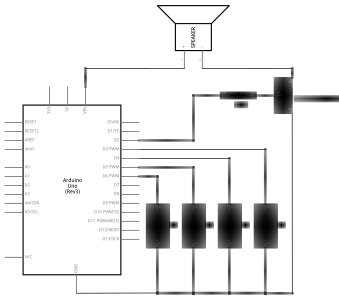
\includegraphics[width=0.75\textwidth]{images/arduino.png}
    \end{center}
    \caption[Circuit design for the Arduino box]{
        Circuit design for the Arduino box.
    }\label{fig:arduino_circuit}
\end{figure}

\begin{figure}[p]
    \begin{center}
        \includegraphics[width=\textwidth]{images/arduino_photo.jpg}
        \includegraphics[width=\textwidth]{images/box_photo.jpg}
    \end{center}
    \caption[Building the dome Arduino box]{
        Building the dome Arduino box in the lab in Sheffield.\\
        Top: Testing the circuit design with the Arduino (circuit board in the back) and two of the dome switches: a magnetic security switch (grey blocks on the left) and a Honeywell limit switch (cyan unit in the centre, with the cover and arm detached).\\
        Bottom: The completed box, showing the Arduino, power and ethernet cables, siren, and one of the four switches.
    }\label{fig:arduino_wip}
\end{figure}

\newpage

\begin{figure}[p]
    \begin{center}
        \includegraphics[width=0.75\textwidth]{images/box_installed_photo.jpg}
    \end{center}
    \caption[The Arduino box installed in the GOTO dome]{
        The Arduino box installed in the GOTO dome during my first trip to La Palma in March 2017. This photo was taken before the cover and cables were attached.
    }\label{fig:arduino_installed}
\end{figure}

\begin{figure}[p]
    \begin{center}
        \includegraphics[width=0.75\textwidth]{images/box_installed_photo2.jpg}
    \end{center}
    \caption[The Arduino box and quick-close button in the GOTO dome]{
        The Arduino box and yellow quick-close button in the GOTO dome, attached to the southern pillar under the dome drive. The cables run to the computer rack which is just off to the left of the photo.
    }\label{fig:arduino_button_dome}
\end{figure}

\newpage

\begin{figure}[p]
    \begin{center}
        \includegraphics[width=0.8\textwidth]{images/dome_sensor_1.jpg}
        \includegraphics[width=0.8\textwidth]{images/dome_sensor_2.jpg}
        \includegraphics[width=0.8\textwidth]{images/dome_sensor_3.jpg}
    \end{center}
    \caption[Additional sensors added to the dome]{
        Additional sensors added to the dome during the March 2017 trip:\\
        Top: One of the two limit switches added to detect when the dome is fully open.\\
        Middle: The magnetic switch added to detect when the dome is fully closed.\\
        Bottom: The magnetic switch added to the dome hatch to detect if it is open or closed.
    }\label{fig:dome_switches}
\end{figure}

\clearpage

Using a combination of these new switches and the PLC output is is possible for the dome daemon to build up a complete status of the dome. The software implementation of this is described in \aref{sec:dome}. Having a sensor on the hatch also allowed it to be added as a conditions flag as described in \aref{sec:conditions_flags}, meaning the pilot will stop and report if the hatch is open when in robotic mode. As of yet the hatch flag or in-dome buttons have not been needed in an emergency, however they are important as an insurance policy just in case. It is anticipated that the same work will need to be done in the second GOTO dome when it is commissioned. Comments have also been passed on to Astrohaven to suggest they could include some of the features in their own stock hardware, for example a built-in siren that could be optionally sounded whenever the dome is moving.

One further addition to the GOTO dome should be mentioned: the ``heartbeat'' monitor designed and installed by Paul Chote at Warwick. As described in \aref{sec:dome}, in the event that the dome daemon crashes or the control NUC itself fails for whatever reason the dome would be left vulnerable --- especially if it was already open. As a backup Paul created his own Arduino system that connects to the dome PLC and will send it commands to close in the event that it does not receive a regular signal from the dome daemon. This system was installed into the GOTO dome in April 2018, along with the other Warwick telescopes on the site, and was one of the final stages required before GOTO could safely leave the commissioning phase and not require an on-site monitor. As a similar new addition to the domes Paul used some of the ideas from the system outlined here, for example integrating a siren into the W1m unit. When the second GOTO dome is commissioned we will consider if the two systems could be merged.

\end{colsection}

% ~~~~~~~~~~~~~~~~~~~~

\newpage
\subsection{Commissioning challenges}
\label{sec:challenges}
\begin{colsection}

Not mentioned: SiTech TCP/IP, Camera speed-up

filter wheel serials

Camera readout not storing

Dec drive failing

Mount balancing

Dome stutter and falling open in the ice


\end{colsection}

% ~~~~~~~~~~~~~~~~~~~~

\end{colsection}

% ########################################

\newpage
\section{Developing observing routines}
\label{sec:obs_scripts}
\begin{colsection}

% ~~~~~~~~~~~~~~~~~~~~

\begin{colsection}

\todo{WIP}

\end{colsection}

% ~~~~~~~~~~~~~~~~~~~~

\subsection{Taking flat fields}
\label{sec:flats}
\begin{colsection}

\todo{WIP}
\citep{flats}

\end{colsection}

% ~~~~~~~~~~~~~~~~~~~~

\subsection{Focusing the telescopes}
\label{sec:autofocus}
\begin{colsection}

\todo{WIP}
\citep{autofocus}

\end{colsection}

% ~~~~~~~~~~~~~~~~~~~~

\end{colsection}

% ########################################

\newpage
\section{System performance}
\label{sec:results}
\begin{colsection}

% ~~~~~~~~~~~~~~~~~~~~

\begin{colsection}

\todo{WIP}

\end{colsection}

% ~~~~~~~~~~~~~~~~~~~~

\subsection{Hardware control}
\label{sec:hardware_results}
\begin{colsection}

\todo{WIP}

\end{colsection}

% ~~~~~~~~~~~~~~~~~~~~

\subsection{The all-sky survey}
\label{sec:survey_results}
\begin{colsection}

\todo{WIP}

\end{colsection}

% ~~~~~~~~~~~~~~~~~~~~

\subsection{Gravitational wave observations}
\label{sec:gw_results}
\begin{colsection}

\todo{WIP}

\end{colsection}

% ~~~~~~~~~~~~~~~~~~~~

\subsection{Other transient follow-up}
\label{sec:other_results}
\begin{colsection}

\todo{WIP}

\end{colsection}

% ~~~~~~~~~~~~~~~~~~~~

\end{colsection}

% ########################################
